%%%%%%%%%%%%%%%%%%%%%%%%%%%%%%%%%%%%%%%%%%%%%%%%%%%%%%%
% A template for Wiley article submissions developed by 
% Overleaf for the Overleaf-Wiley pilot which ran 
% during 2017 and 2018.
% 
% This template is no longer supported, but is provided
% for historical reference. Last updated January 2019.
%
% Please note that whilst this template provides a 
% preview of the typeset manuscript for submission, it 
% will not necessarily be the final publication layout.
%
% Document class options:
% =======================
% blind: Anonymise all author, affiliation, correspondence
%        and funding information.
%
% lineno: Adds line numbers.
%
% serif: Sets the body font to be serif. 
%
% twocolumn: Sets the body text in two-column layout. 
% 
% num-refs: Uses numerical citation and references style 
%           (Vancouver-authoryear).
%
% alpha-refs: Uses author-year citation and references style
%             (rss).
%
% Using other bibliography styles:
% =======================
%
% To specify a different bibiography style
%
% 1) Do not use either num-refs or alpha-refs in documentclass.
% 2) Load natbib package with the options set as needed.
% 3) Use the \bibliographystyle command to specify the style
% 
% Included NJD styles are: 
%   WileyNJD-ACS
%   WileyNJD-AMA
%   WileyNJD-AMS
%   WileyNJD-APA
%   WileyNJD-Harvard
%   WileyNJD-VANCOUVER
%
% or you may upload an alternative .bst file 
% (if requested by the journal).
%
% Examples:
% =======================
%% Example: Using numerical, sort-by-authors citations.


\documentclass[num-refs]{wiley-article}
%% Example: Using author-year citations and anonymising submission
% \documentclass[blind,alpha-refs]{wiley-article}

%% Example: Using unsrtnat for numerical, in-sequence citations
%\documentclass{wiley-article}
%\usepackage[numbers]{natbib}
%\bibliographystyle{unsrtnat}

%Citation style from another project
%\usepackage[citestyle=numeric,style=numeric,backend=biber]{biblatex}
%% Example: Using WileyNJD-AMA reference style and superscript
%%          citations, two-column and serif fonts for AIChE
%\documentclass[serif,twocolumn,lineno]{wiley-article}
\bibliographystyle{WileyNJD-AMA}
% \makeatletter
% \renewcommand{\@biblabel}[1]{#1.}
% \makeatother

% Add additional packages here if required
\usepackage{natbib}
\usepackage{siunitx}
\graphicspath{{./images/}}
\usepackage{wrapfig}
% Update article type if known
\papertype{Original Article}
% Include section in journal if known, otherwise delete
\paperfield{Organic chemistry synthesis}

\title{Synthesis of \texorpdfstring{H\textsubscript{2}}-TPP and its metallation to Zn-TPP}

% List abbreviations here, if any. Please note that it is preferred that abbreviations be defined at the first instance they appear in the text, rather than creating an abbreviations list.
\abbrevs{\texorpdfstring{H\textsubscript{2}}-TPP, 5,10,15,20-meso-tetraphenylporhyrin.}

% Include full author names and degrees, when required by the journal.
% Use the \authfn to add symbols for additional footnotes and present addresses, if any. Usually start with 1 for notes about author contributions; then continuing with 2 etc if any author has a different present address.
\author[1\authfn{1}]{Matteo Finco*, Nicola Milani}


% Include full affiliation details for all authors
\affil[1]{DiSC, Università degli Studi di Padova, Padova, Italy, 35131, Italy}

\corremail{matteo.finco.3@studenti.unipd.it}
% Include the name of the author that should appear in the running header
\runningauthor{Matteo Finco}

\begin{document}

\begin{frontmatter}
\maketitle

\begin{abstract}

% Please include a maximum of seven keywords
\keywords{tetraphenylporphyrin, TPP, Zn-TPP}
\end{abstract}

\end{frontmatter}

\section{Introduction}
\begin{wrapfigure}{L}{0.35\textwidth}
    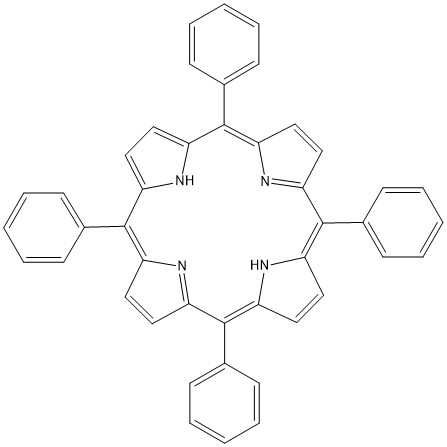
\includegraphics[width=0.3\textwidth]{TPP}
    \caption{TPP structure}
    \label{TPP-structure}
\end{wrapfigure}
Porhyrins represent an obiquitous class of molecules that plays a crucial role biochemistry for oxygen transport\citep{hardison_evolution_2012}, storage\citep{kendrew_three-dimensional_1958} and catalysis as well as electron transfer\citep{keilin_cytochrome_1925}.\\
Therefore, extensive efforts have been put into the exploration of the functionalities obtainable by artificially synthesized porphyrins.\\
The biomimetic electrocatalysis\cite{facchin_oxygen_2021,liang_porphyrin-based_2021} and cancer treatment and diagnosis\cite{wang_recent_2021} represent two outstanding examples among all the use cases in which porphyrins have been successfully deployed.
Numerous works elaborate the further functionalization of \textit{meso}-tetraphenylporphyrin\cite{silva_porphyrins_2006} in order to realize functional materials. \\
However, to date the scale up in complex porphyrins production and broad commercial application is prevented by the production costs which are primarily led up by the expensiveness of reactants, inefficient and unreliable synthesis.
In the following work, a simple synthesis route for 5,10,15,20-mesotetraphenylporhyrin is detailed and its products are critically discussed either for the \texorpdfstring{H\textsubscript{2}}-TPP and the metallated Zn-TPP.
\newpage

\twocolumn
\section{Methods}
\begin{figure*}[t!]
        \centering
        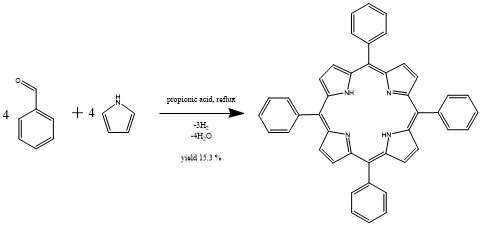
\includegraphics[width=0.6\textwidth]{reaction}
        \caption{Reaction scheme for \textit{meso}-TPP synthesis through condensation in acidic medium.}
        \label{reaction}
\end{figure*}
The synthesis proposed for \textit{meso}-tetraphenylporphyrin is a multistep electrophilic aromatic substitution between the electrophilic carboxilic group of protonated benzaldehyde on the aromatic ring of pyrrole which is summarized in Fig.\ref{reaction}.
The protonation of benzaldehyde implies that the reaction is performed in acidic environment, and its protonated form is stabilized by the resonance forms reported in Fig.\ref{res-benz}.\\
\begin{figure*}[b!]
    \centering
    \begin{subfigure}
        \centering
        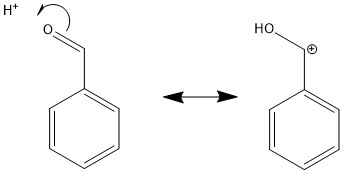
\includegraphics[width=0.3\textwidth]{resonance-benzaldehyde}
        \caption{Resonance forms of benzaldehyde in acidic environment.}
        \label{res-benz}
    \end{subfigure}
    \begin{subfigure}
        \centering
        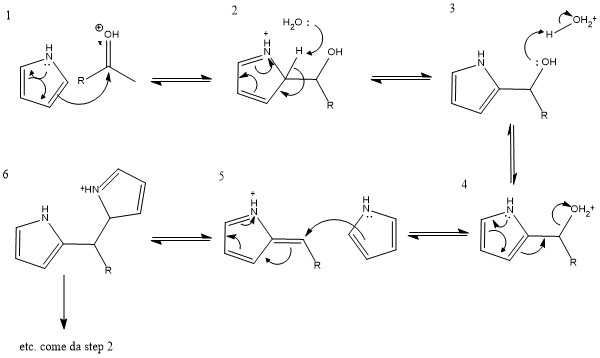
\includegraphics[width=0.5\textwidth]{mechanism}
        \caption{Reaction mechanism for electrophilic substitution on the pyrrolic ring by aldehyde groups.}
        \label{mechanism}
    \end{subfigure}
\end{figure*}
This route is called Rothemund synthesis and proceeds through the repetition of the six steps in Fig.\ref{mechanism} thanks to the driving force provided by the stability of the wide aromatic system.
The reaction consists in multiple condensations occurring at the addition of each unit to the porhyrinic ring.
The first step consist in the electrophylic attack of the protonated aldehyde to the pyrrolic ring.
Then, the pyrrolic ring extracts the positive charge and gets deprotonated in the second step.
The re-protonation of the carbonilic group by the acidic environment forms the leaving group -OH$_{2}$$^{+}$ which causes the condensation of the reagents and the relocaliization of the positive charge on the nitrogen atom by the misplacing of its lone pair into the pyrrolic ring.
The methynic bridge is instaurated by the electrophyle attack of the insaturated bond and the concerted relocation of the positive charge into the newly added pyrrolic ring.
\break
The metallation of the free base porhyrin is operated by the reaction in reflux conditions with zinc acetate as reported in Fig. \ref{metalation}.
\begin{figure*}
    \centering
    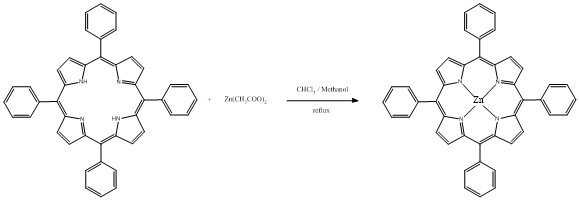
\includegraphics[width=0.8\textwidth]{Zn-TPP reaction}
    \caption{Reaction scheme for the metallation of the free base porphyrin.}
    \label{metalation}
\end{figure*}
The use of chloroform is necessary for the solvation of the freebase porphyrin, while methanol solvates the zinc acetate.
The metallation of the free base porphyrin is allowed by its deprotonation which is allowed by the basic behaviour of the acetate anion.
Then, the Zn(II) cation is coordinated by the four nitrogen atoms.

%%%%%%%%%%%%%%%%RESULTS AND DISCUSSION%%%%%%%%%%%%%%%

\section{Results and Discussions}
In the following section, the characterization results are presented and discussed for both, the free base and the metallated porphyrin.
\subsection{\textit{In situ} characterizations}
The reactions were monitored using Thin Layer Chromatography.
In Fig. \ref{tlc-h2tpp} it is possible to see that the reaction already had occurred by the time of the first control, which corresponds to around 5 minutes of reaction time.
This can be affirmed since the control TLC performed after 30 minutes of reaction time also against a commercial standard, exhibited the same features.
It must be noted that the R$_{f}$ of the tested samples appear to shift to higher values.
The reason of which might be found in two possible phenomena, namely the change in eluent composition due to higher vapor pressure of petroleum ether compared to methanol and the excessive eluent run that was performed on the second plate.
Indeed, the fact that the second plate had the eluent almost to its edge might have caused a distortion of the R$_{f}$ in excess.
In the meanwhile, the instability in composition of the eluent might explain the shift in relative differences of the R$_{f}$ coefficients between benzaldehyde and pyrrole, since their difference in R$_{f}$ changes from 14\% to 9\%.

At the end of the synthesis, the yield was estimated to be 15.3\%, which amounted to the synthesis of 0.339 g of product against the 2.21 g expected if the reaction had been quantitative and limited by pyrrole, the limiting reactant.
The metallation of the free base porphyrin was monitored once again by the use of TLC plates 2, 5 and 25 minutes since the beginning of the reaction.
The results of which can be observed in the Fig.\ref{TLC-Zn-TPP}.\\
\begin{figure*}[t!]
    \centering
    \begin{subfigure}
        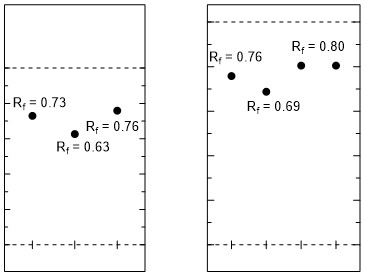
\includegraphics[width=0.3\textwidth]{TLC-h2-TPP}
        \caption{On the left, the TLC run performed 5 minutes after the addition of the reagents to the flask. The spots from left to right are corresponding to benzaldehyde, pyrrole and the reaction solution. On the right, the TLC run performed 30 minutes after the addition of the reagents to the flask. The spots from left to right are corresponding to benzaldehyde, pyrrole, commercial H$_{2}$-TPP and the reaction solution.}
        \label{tlc-h2tpp}
    \end{subfigure}
    \begin{subfigure}
        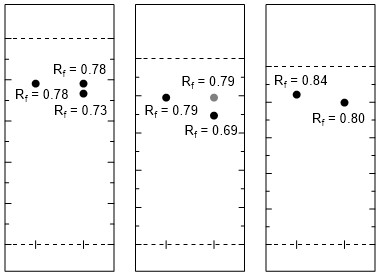
\includegraphics[width=0.3\textwidth]{TLC-Zn-TPP}
        \caption{The spots are corresponding to the prepared H$_{2}$-TPP on the left and the reaction solution on the right, respectively sampled 2, 5 and 25 minutes after the beginning of the reaction.}
        \label{TLC-Zn-TPP}
    \end{subfigure}
\end{figure*}
%%%%%%%%%% Presentation of results obtained by other studies
\subsection{\textit{$^{1}$H NMR} characterization}
%Discussing the results of NMR --- Spectra and motivations
For this analysis, the spectra found in the work of \citet{anjali_zinc-tetraphenylporphyrin_2020} has been used as a literature source for displaying the interpretation of NMR spectra.
It must be pointed out that they incorrectly assign the \textbf{b} and \textbf{d} positions, therefore the presented spectra have been amended.
The execution of $^{1}$H NMR on the expected free base TPP returned five main signals (see Fig.\ref{NMR-H2-TPP}), which are attributed as follows.
The most shielded at -2.713 ppm is attributed to NH protons, due to the electronrich character of the pyrrolic ring. 
In addition, its absence of multiplicity suggests the absence of hydrogen atoms in neighbouring positions, a condition that is only verified by NH protons in the structure of the target TPP.
The remaining peaks are all placed in the aromatic reagion. 
The attributions indicated are based on the idea that the proximity to the porphyrinic ring removes shielding, in order to distinguish b and c positions, and that pyrrolic protons have a higher shift than the phenylic ones, allowing the attribution of the d proton signal.
The integrated signals confirm once more the attribution of signals, since the \textbf{b} positions are in 3/2 with the ones in \textbf{c} and \textbf{d} positions.
It is noticeable that the slight shift difference expected between protons placed in the phenyl ring in \textit{meta} and \textit{para} positions, doesn't allow an effective discrimination of the two contributions.
Finally, it is noted that TMS is found in very close proximity to its expected shift of 0.
The fact that the features found can all be interpreted by the expected signals, suggest a good degree of purity of the synthesized compound and that the target synthesis was performed successfully.\\
Similarly, the spectrum of the product of metallation has been studied by $^{1}$H NMR, see Fig.\ref{NMR-Zn-TPP}.
In this case, the very same peaks are observed, besides the ones corresponding to the NH protons.
This allows to verify that protons have been removed completely from that position, but doesn't allow to verify the presence of Zn atoms coordinated by the porphyrinic system.
\begin{figure}
    \centering
    \begin{subfigure}
        \centering
        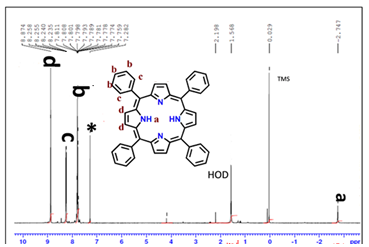
\includegraphics[width=0.45\textwidth]{1H-NMR-H2-TPP}
        \caption{$^{1}$H-NMR of Zn-TPP in TMS.}
        \label{NMR-H2-TPP}
    \end{subfigure}
    \begin{subfigure}
        \centering
        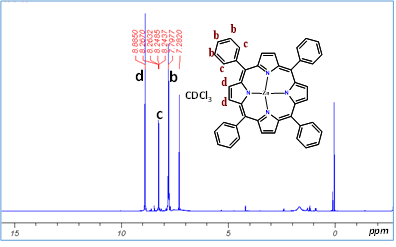
\includegraphics[width=0.5\textwidth]{1H-NMR-Zn-TPP}
        \caption{$^{1}$H-NMR of Zn-TPP in chloroform.}
        \label{NMR-Zn-TPP}
    \end{subfigure}
\end{figure}
\subsection{\textit{ESI-MS} characterization}
%Discussing the results of MS --- Spectra and motivations

\subsection{Study case}
%Presenting an insightful paper
\section{Conclusions}
\section{Experimental}
Reagents were loaded in a round-bottomed flask containing 40 mL of propionic acid.
Firstly, the flask was placed in a heating mantle mounted with an Allihn condenser on top and heated to boil the acid.
The reagents, consisting in 1.65 mL (15.75 mmol) of benzaldehyde and 1 mL of pyrrole (14.4 mmol), were loaded from the upper end of the condenser at the same time to avoid pyrrole polymerization.
Therefore, a small excess of benzaldehyde was used in order to prevent polymerization of the pyrrole into polypyrrole \\
Following, the condenser's walls were wahed with 10 mL of propionic acid to ensure quantitative transfer of the reagents to the flask.
The reaction was driven in reflux conditions for 30 minutes and was monitored through TLC at the beginning and after 30 minutes of reflux.
All the TLCs were performed using as eluent a solution of petroleum ether and ethyl acetate in 3:1 volumetric ratio.
A purple precipitate formed in the flask and upon cooling it was filtered from the solvent.
The filtration was performed using a gootch sieve with a porosity of 3 mounted on Buchner flask connected to a vacuum line.
Subsequently, the solid was washed from propionic acid using methanol, due to the higher volatility of the latter.
The purple crystals, which can be seen in Fig.\ref{pic-tpp}, were removed from the porous sieve with a spatula and transferred into a vial which had been previously weighted.
The product was weighted through the use of a digital scale in order to estimate the reaction yield and a TLC was performed against a commercial standard to ensure successful synthesis.\\
\begin{figure}[h]
    \centering
    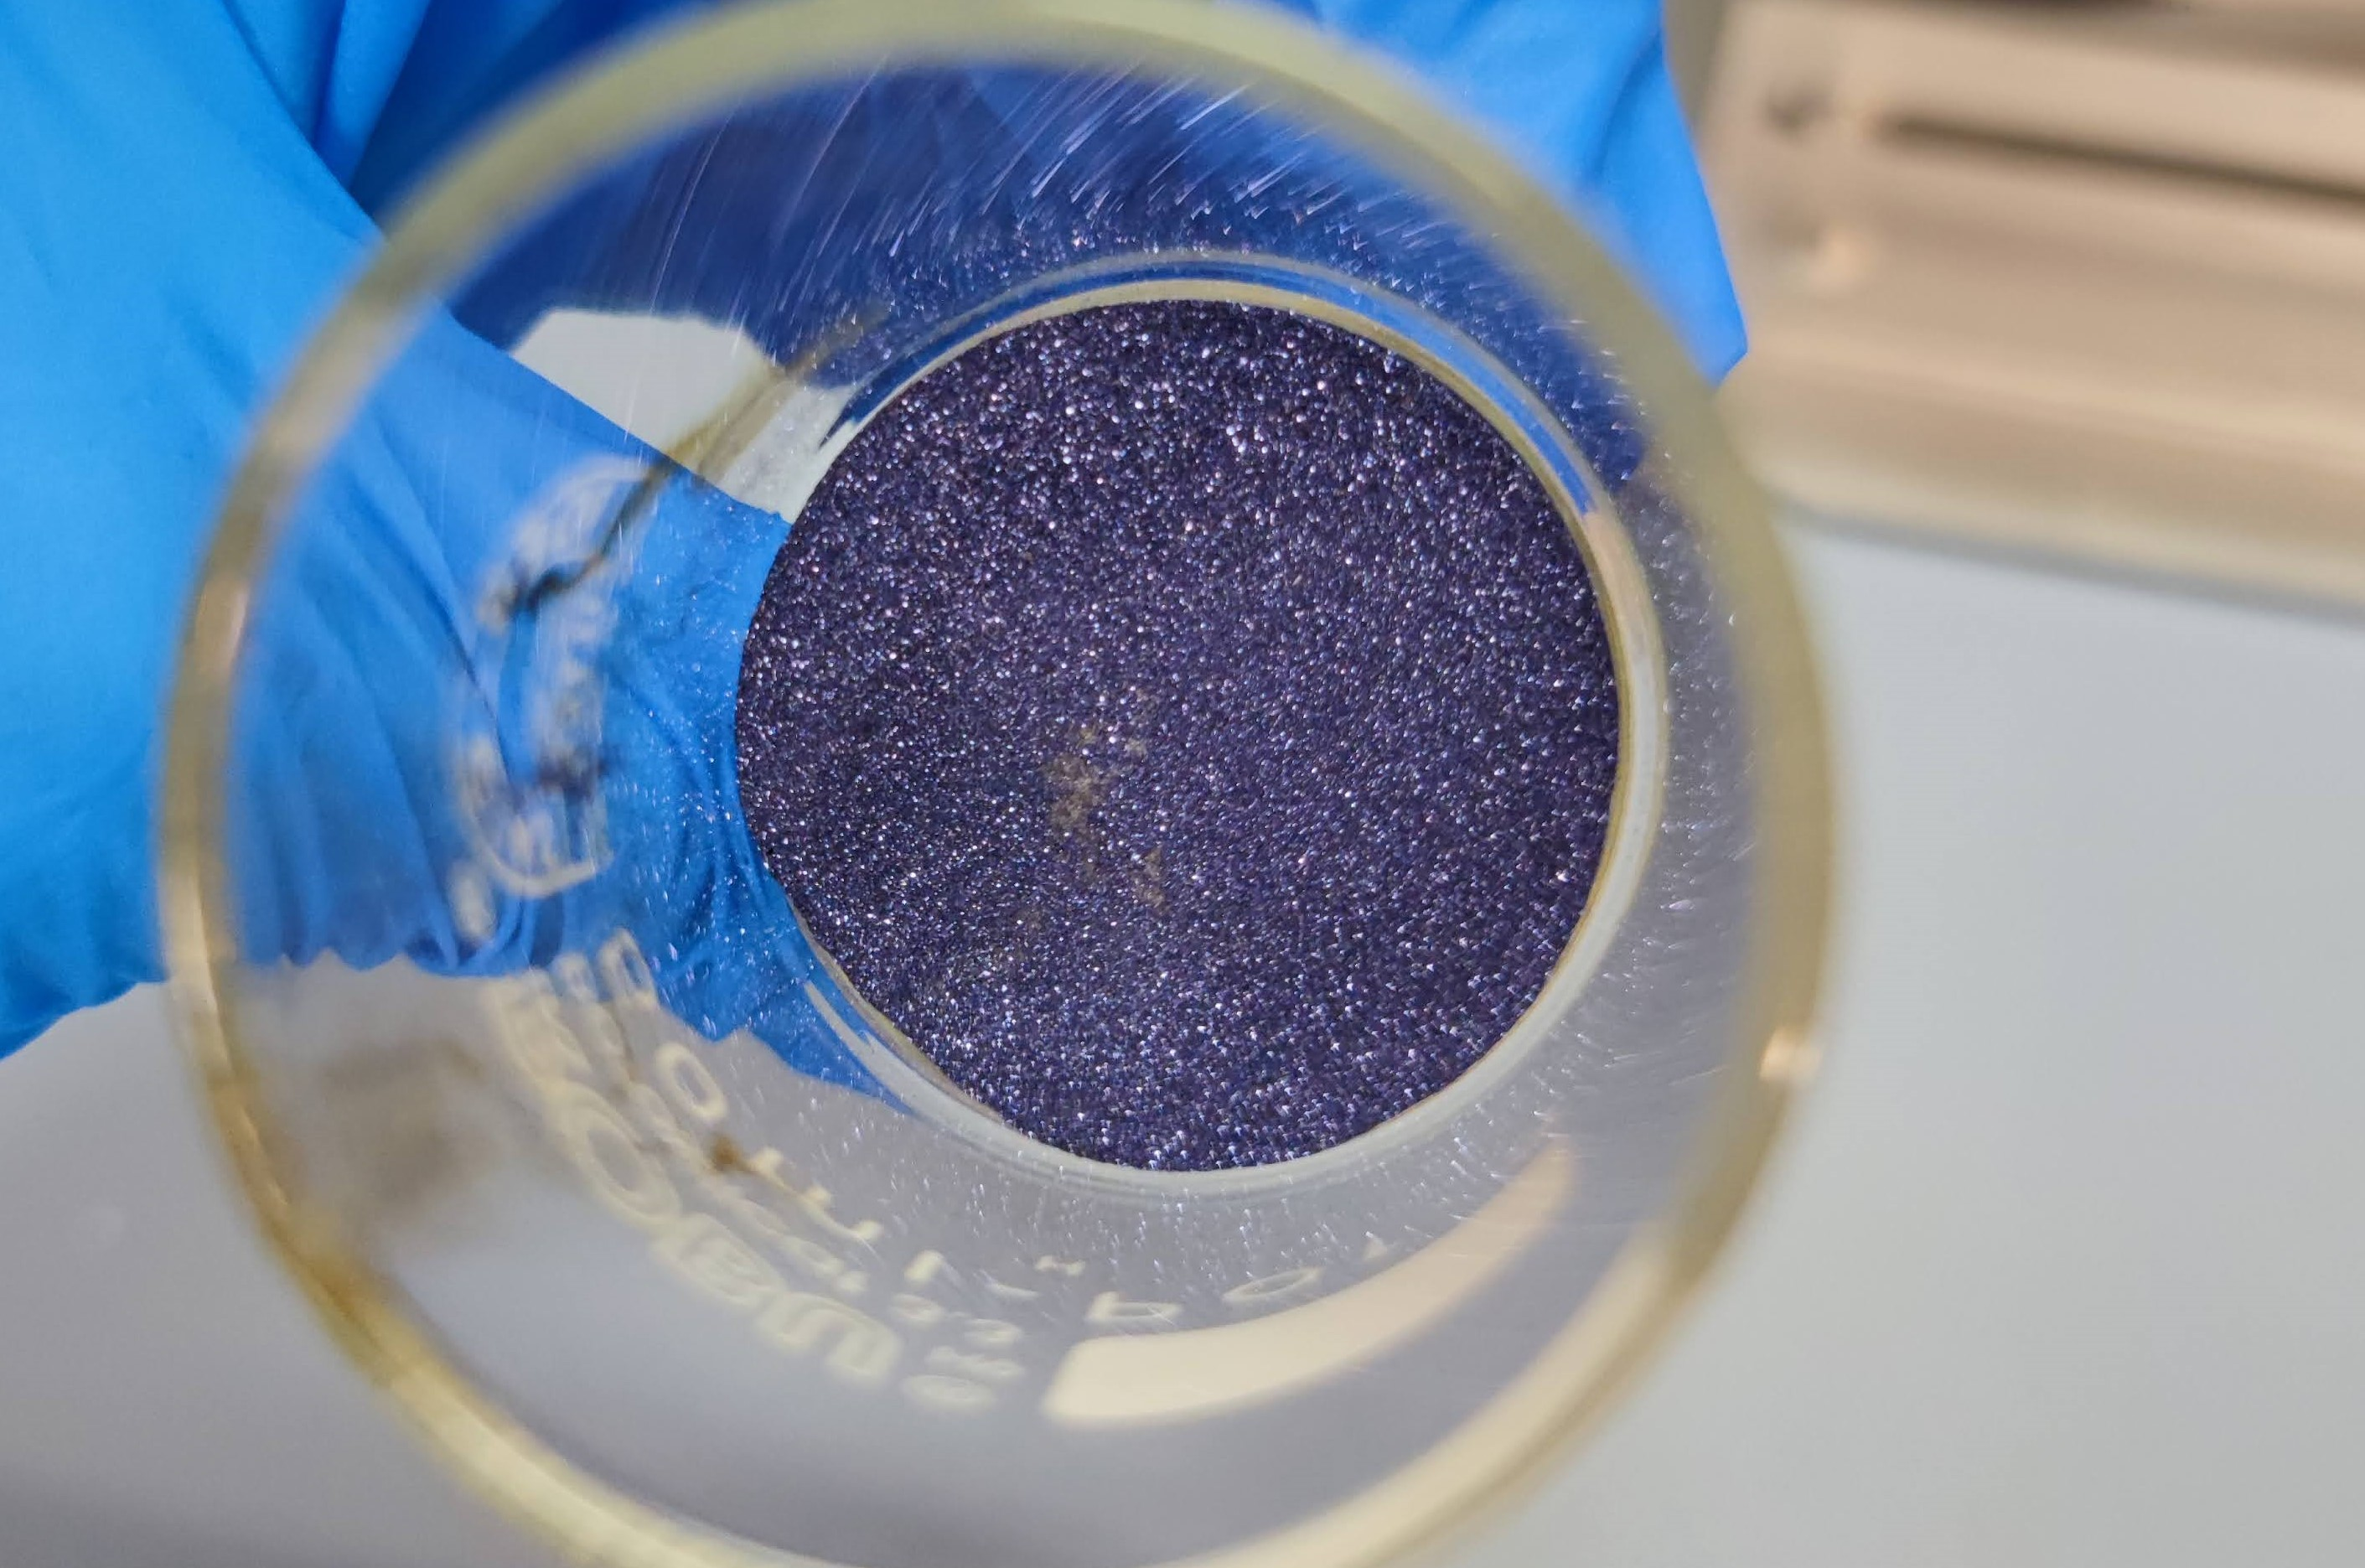
\includegraphics[width=0.4\textwidth]{photo-tpp}
    \caption{Picture portraying the H$_{2}$-TPP crystals collected on the sieve.}
    \label{pic-tpp}
\end{figure}
\break
The metallation of the as-synthesized porphyrin was realized on 200 mg of the sample.
The intermediate product was weighted on a watch glass and then trasferred into a round-bottomed flask alongside with 20 mL of chloroform and heated using a heating mantle.
A volume of 4 mL of a saturated solution of zinc acetate in methanol was then added to the flask and reflux conditions were imposed using an Allihn condenser for 30 minutes.
Also this reaction was monitored through TLC of H$_{2}$-TPP, the starting solution and the reaction solution after 2, 5 and 25 minutes after mixing the reagents.
In order to avoid the streaking of the spots, the samples from the reaction solution were diluted in chloroform before placing on the TLC plate.\\
\break
At this point, the purification of Zn-TPP is needed in order to separate the product from zinc acetate precursor.
This is achieved through the employment of a separating funnel and use of water as the extracting phase for zinc acetate.
The separation was repeated twice using each time 20 mL of milliQ water.
Furthermore, anhydrification of the chloroform containing Zn-TPP was undertaken by the addition of abundant Na$_{2}$SO$_{4}$ powder.
The sodium sulfate is added until the newly added powder stops aggregating, testifying the lack of water.
The insoluble powder has been filtered from the organic solvent using a paper filter folded to fit in a funnel.
The filtered liquid, containing dissolved Zn-TPP, was collected in a 100 mL round-bottomed flask.
Ultimately, the flask was placed in a rotavapor system to evaporate the solvent and enable the collection of the solid product.
The reaction yield was again estimated by the use of a digital scale and the product was transferred into a vial before undergoing the analysis described ....

\section*{acknowledgements}
The contributions of former students in collecting the experimental characterization of their sample has been crucial for validating the synthesis proposed in this work.
\section*{conflict of interest}
The author reports to have a personal interest in the positive outcome of the research work.
\section*{Supporting Information}
A GitHub repository hosts the complete file collection produced as part of this coursework.
It can be found at https://github.com/EC-Finco/Porphyrins-report.
\printendnotes

% Submissions are not required to reflect the precise reference formatting of the journal (use of italics, bold etc.), however it is important that all key elements of each reference are included.
\bibliography{rifporphyrin}
\graphicalabstract{example-image-1x1}{Please check the journal's author guidelines for whether a graphical abstract, key points, new findings, or other items are required for display in the Table of Contents.}
\end{document}